%%-----------------------------------------------------
%%-----------------------------------------------------
\section{Scratch: Enseña a programar}


%-----------------------    ---------------------------------


\begin{frame}
\frametitle{}

\begin{center}
  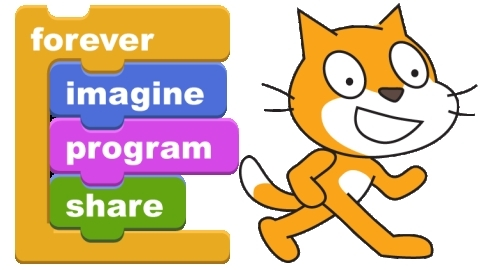
\includegraphics[width=8cm]{figs/scratch.jpg}
\end{center}


\begin{flushright}
{\tiny
http://canaltic.com/vr/manual/scratch001.jpg
}
\end{flushright}

\end{frame}


%-----------------------    ---------------------------------

\begin{frame}
\frametitle{Scratch y AppInventor}

\begin{itemize}
   \item Fruto de la preocupación de falta de interés por la programación
   \item Es un subconjunto de lo que se conoce como potenciaciación del pensamiento computacional
   \item Hay 10 veces más líneas de código en un coche (de gama alta, hoy) que en un avión
   \item Programación visual, orientada a la enseñanza
   \item Las plataformas permiten compartir y remezclar
\end{itemize}

\end{frame}



%-----------------------    ---------------------------------

\begin{frame}
\frametitle{}

\begin{center}
  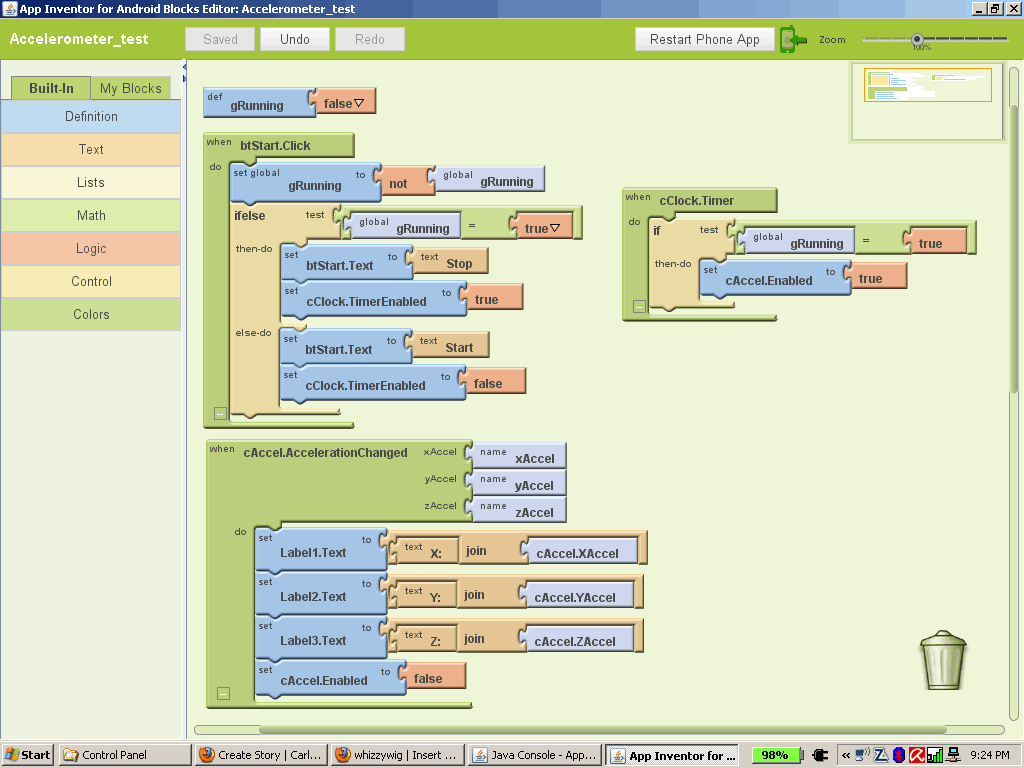
\includegraphics[width=10cm]{figs/appInventor.png}
\end{center}


\begin{flushright}
{\tiny
http://www.carloslabs.com/files/app-inventor/accelerometer-test.gif
}
\end{flushright}

\end{frame}


